\documentclass[fontsize=12pt]{scrartcl}
\usepackage[ngerman]{babel}
\usepackage[utf8]{inputenc}
%\usepackage[latin1]{inputenc}
\usepackage{amsmath}
\usepackage{amstext}
\usepackage{amssymb}
\usepackage{stmaryrd}
\usepackage{verbatim}
\usepackage{mathrsfs}
\usepackage{extarrows}
\usepackage[arrow, matrix, curve]{xy}
\usepackage[centering,includeheadfoot,margin=2cm]{geometry}
\usepackage{gensymb}
\usepackage{graphicx}
\usepackage{framed}
\usepackage{xcolor}
\usepackage{float}
\usepackage{graphicx} 
\usepackage{sidecap}
\usepackage{blindtext,wrapfig}
\usepackage{epstopdf}
\usepackage{import}
\usepackage{fancyhdr}
\usepackage{fancybox}
\usepackage{graphicx}
\usepackage{caption}
\usepackage{subcaption}
\DeclareGraphicsRule{.tif}{png}{.png}{`convert #1 `basename #1 .tif`.png} 
\pagestyle{fancy}
\fancyhf{}
\fancyhead[R]{Physiklaisches Praktikum 1}
\fancyhead[L]{Linda Werneck, Gentian Rrafshi}
\fancyfoot[R]{Seite \thepage}
\fancyfoot[L]{\today}

\begin{document}

\begin{minipage}{\textwidth}
\begin{center}\large
\title{E10b Wechselstromwiderstände: Serienschwingkreis \\
		~\\
		~\\
		Assistent: Jonas Binz \\
		Datum Versuchsdurchführung: \\
		29.04.2015}

\author{bearbeitet von\\
		Gruppe 3-031: \\
		Linda Werneck Matrnr. 2901495 \\
		Gentian Rrafshi Matrnr. 2721617 }
\date{\today}

\maketitle

\end{center}
\end{minipage}

\newpage

\tableofcontents

\newpage
\noindent

\section{ Versuchsziel}

Versuchsziel ist die Bestimmung der Resonanzfrequenz, die Berechnung eines frequenzabhängigen Widerstands in einem Serien- und Parallelschwingkreis und die Berechnung der Phasenverschiebung bzw. der Phase. Dazu verwendet man die Wheatstone’sche Brücke.

\section{ Grundlagen}

\subsection{komplexe Wechselstromwiderstände}

Grundlage dieses Versuchs ist die Wechselstrom, welcher Auswirkung auf Spule und Kondensator hat. Diese werden nun zu induktiven und kapazitiven Widerständen. Diese sind frequenzabhängig und es lassen sich folgende Beziehungen feststellen: 
\begin{align*}
 U &= L \cdot \frac{d}{dt} I = L \cdot \dot{I} \\
 I &= C \cdot \frac{d}{dt} U = C \cdot \dot{U}
\end{align*}
\noindent
Diese DGLs lassen sich mit den Ansätzen $I(t)=I_0 \cdot e^{i\omega t}$ und $U(t) = U_0 \cdot e^{i\omega t}$ lösen. Es ergibt sich dadurch:
\begin{align*}
U &= L \cdot \dot{I} = L \cdot \frac{d}{dt}{I_0 \cdot e^{i\omega t} } = i\omega L \cdot I_0 \cdot e^{i\omega t} =  i\omega L \cdot I  \\
 I &= C \cdot \dot{U} = C \cdot \frac{d}{dt} U_0 \cdot e^{i\omega t} = i\omega  C \cdot U_0 \cdot e^{i\omega t} =  i\omega  C \cdot U
\end{align*}
\noindent
Dadurch ergibt sich durch einfaches Umstellen nach U die komplexen Widerstände $Z_C = \frac{1}{i\omega C}$ und $Z_L= i \omega L$.$^{\cite{1}}$

\subsection{Das RC-Glied}

RC-Glieder sind eine Kombination aus ohmschen Widerständen R und kapazitiven Widerständen C. In der Reihendarstellung ergibt sich für den komplexen Wechselstromwiderstand: 
\begin{equation*}
Z_x = R_{\Omega} + \frac{1}{i\omega C}
\end{equation*}
und in Paralleldarstellung ergibt sich für den komplexen Wechselstromwiderstand für $Y=\frac{1}{Z}$ als den Leitwert:$^{\cite{1}}$
\begin{equation*}
Y_x = \frac{1}{R_{\omega}} + i\omega C
\end{equation*}

\newpage
\subsection{Serien-/Parallelschwingkreis}

Ganz analog zu RC-Glied lässt sich auch ein LC-Glied kombinieren, Hierbei \glqq pendelt \grqq   die eingespeicherte Energie zwischen den Kondensator und der Spule und zurück, pendelt also periodisch. \\
~\\
Für eine Serienschwingkreis mit einem ohmschen Widerstand ergibt sich für den Gesamtwiderstand:
\begin{align*}
Z= R_{\Omega} + i\omega L + \frac{1}{i\omega C}
\end{align*}
Hierbei sieht man, dass Z für kleine und große Frequenzen gegen unendlich strebt. Das Minimum erreicht $Z$ genau an der sogenannten Resonanzfrequenz.$^{\cite{1}}$

\section{Versuchsaufbau und Durchführung}

\subsection{Benötigte Geräte}

\begin{itemize}
\item[•] Gleich große Widerstände $(R_{2}=R_{3}=R_{4}=4,7\Omega)$
\item[•] Frequenzgenerator $(U_{n})$
\item[•] Stufenkondensator $(C_{n})$
\item[•] Widerstandsdekaden $(R_{n})$
\item[•] Differenzverstärker (V)
\item[•] Komplexer Widerstand $(Z_{x})$
\item[•] Kabel
\item[•] Oszilloskop
\end{itemize}

\subsection{Versuchsaufbau und -Durchführung}

\begin{figure}[h]
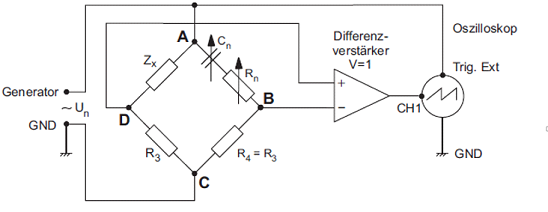
\includegraphics[scale=0.7]{Graphik/Versuchsaufbau}
\caption{Versuchsaufbau$^{\cite{A}}$}
\end{figure}
~\\
Der Versuch wird zunächst nach Abbildung 1 mit den in 3.1 genannten Geräten aufgebaut, angeschaltet und das Bild getriggert. \\
~\\
Um im Vorversuch die Resonanzfrequenz zu bestimmen müssen die Punkte A und B überbrückt werden. Die Generatorfrequenz wird variiert und dabei auf dem Oszilloskop die Spannung des Serienschwingkreises beobachtet. Die Frequenz, für welche die Spannung ein Minimum erreicht, ist die Resonanzfrequenz. \\
~\\
Der erste Teil des Versuchs kann durchgeführt werden. Dabei stellt man eine spezielle Frequenz am Generator ein und verändert die Einstellungen am Stufenkondensator und Widerstandsdekaden so, dass die Spannung des Serienschwingkreises minimal wird. Die Messwerte werden in Abhängigkeit der Frequenz notiert. Man misst bei 10 verschiedenen Frequenzen zwischen 0,2 kHz und der Resonanzfrequenz, wobei die Abstände zwischen den Frequenzen kleiner werden, je näher sie an der Resonanzfrequenz liegen. \\
~\\
Der Versuch muss nun zu einem Parallelschwingkreis nach Abbildung 2 umgebaut werden. \\

\begin{figure}[h]
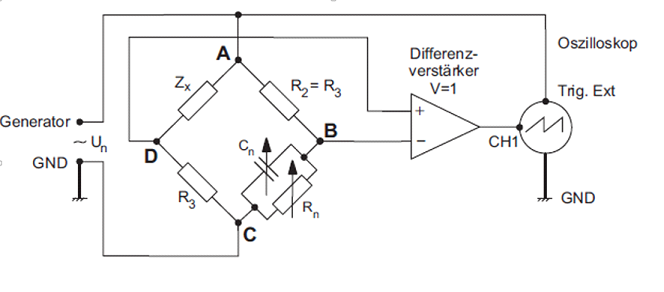
\includegraphics[scale=0.7]{Graphik/Versuchsaufbau2}
\caption{Versuchsaufbau$^{\cite{B}}$}
\end{figure}
~\\
Der zweite Teil des Versuchs wird analog zum ersten Teil durchgeführt, das heißt es werden Frequenzen im Bereich zwischen der Resonanzfrequenz und 8 kHz an dem Generator eingestellt und die Einstellungen am Stufenkondensator und Widerstandsdekaden so lange variiert, bis die Spannung des Schwingkreises ein Minimum erreicht hat. Die Messwerte werden notiert.
\newpage
\section{ Formeln}

\subsection{Formeln für Berechnung des Scheinwiderstandes}

\begin{equation}
|Z_{x}|= \sqrt{[\Re(Z_{x})]^2 +[\Im(Z_{x})]^2}
\end{equation}
\noindent
$\Re(Z_{x})$: 	Realteil des Scheinwiderstands \\
$\Im(Z_{x})$:	Imaginärteil des Scheinwiderstands \\


\subsection{Formeln für den Serienschwingkreis:}
\begin{align}
Z_x &=R_n + \frac{1}{i \cdot \omega \cdot C_{n}} \Longrightarrow \\
\Im(Z_{x})&= - \frac{1}{\omega \cdot C_{n}} = - \frac{1}{2 \cdot \pi \cdot f \cdot C_{n}} \\
\Re(Z_x) &= R_n
\end{align}
Hierbei ist $Z_{3}=R_{3}$ und $Z_{4}=R_{4}=R_{3}$\\
$Z_{x}$: 	Scheinwiderstand \\
$R_{n}$: 	Wert des Widerstandsdekaden, Wirkwiderstand \\
$\omega = 	2 \cdot \pi \cdot f $ \\
$f$: 		Frequenz des Generators \\
$i$: 		komplexe Einheit, $i^{2}=-1$ \\
$C_{n}$: 	Wert des Stufenkondensator \\
\subsection{Formeln für den Parallelschwingkreis:}
\begin{align}
Z_{4} &= \frac{1}{ \frac{1}{R_{n}}+i \cdot \omega \cdot C_{n}} \\
Z_x&= \frac{R^2_3}{Z_4} \Longrightarrow \\
\Im(Z_x) &= R^2_3 \cdot \omega \cdot C_n = R^2_3 \cdot 2 \cdot \pi \cdot f \cdot C_n \\
\Re(Z_x) &= \frac{R^2_3}{R_n}
\end{align}
Hierbei ist $Z_{2}=R_{2}$ und $Z_{3}=R_{3}=R_{2}$

\subsection{Formel für Berechnung der Phasenverschiebung $\Phi$}
\begin{align}
\Phi = \arctan\left(\frac{\Im(Z_{x})}{\Re(Z_{x})}\right)
\end{align}
\noindent
$\Phi$ : 	Phasenverschiebung zwischen Blind- und Wirkwiderstand 

\newpage

\section{ Messwerte}
\begin{figure}[h]
\centering
\caption{Messwerte}
\begin{tabular}{|c|c|c|} \hline
Frequenz [kHz]	&kapazitiver Widerstand $C_n$ in [nF]&reeller Widerstand $R_n$ in $[k\Omega]$ \\ \hline	
0,20	&50,00	&2,50 \\ \hline
0,40	&50,00	&2,50 \\ \hline
0,60	&54,00	&1,20 \\ \hline
0,80	&64,00	&1,10 \\ \hline
1,00	&84,00	&1,20 \\ \hline
1,20	&133,00	&1,20 \\ \hline
1,40	&423,00	&1,20 \\ \hline
1,43	&710,00	&1,20 \\ \hline
1,46	&1100,00	&1,20 \\ \hline
1,49	&1100,00	&1,20 \\ \hline		
\multicolumn{1}{c}{Resonanzfrequenz} \\ \hline
1,60	&1,00	&20,20 \\ \hline
1,70	&2,00	&20,20 \\ \hline
1,80	&3,00	&20,20 \\ \hline
2,00	&5,00	&20,20 \\ \hline
2,50	&7,00	&20,20 \\ \hline
3,00	&8,00	&20,20 \\ \hline
4,00	&9,00	&20,20 \\ \hline
5,00	&10,00	&22,00 \\ \hline
6,00	&10,00	&22,00 \\ \hline
8,00	&11,00	&22,00  \\ \hline
\end{tabular} \\
\end{figure}
\newpage

\section{ Auswertung}

Für diesen Versuch mussten wir erst die Resonanzfrequenz in einem Vorversuch ermitteln. Nach langem justieren ergab es sich, dass die Resonanzfrequenz bei $1,5$\,kHz liegt.

\subsection{Berechnung des Scheinwiderstands für den Serienschwingkreis}

Für die Berechnung des Scheinwiderstands werden die Formeln (1),(3) und (4) benötigt. Als Beispiel wird hier einmal eine Rechnung für die Messwerte bei $200\,$Hz aufgeführt. Am Ende der Auswertung sind alle Werte in einer Tabelle zusammengefasst.
\begin{align*}
|\Im(Z_{x})|&= |- \frac{1}{\omega \cdot C_{n}}| = |- \frac{1}{2 \cdot \pi \cdot f \cdot C_{n}}| \\
&= |- \frac{1}{2 \cdot \pi \cdot 200\,\text{Hz} \cdot 50\cdot 10^{-9}\,\text{F}}| = 15923,57\,\Omega \\
~\\
\Re(Z_x) &= R_n = 2500\,\Omega \\
~\\
|Z_{x}|&= \sqrt{[\Re(Z_{x})]^2 +[\Im(Z_{x})]^2} = \sqrt{R_n^2 + (\frac{1}{2 \cdot \pi \cdot f \cdot C_{n}})^2} \\
&= \sqrt{15923,57^2\,\Omega^2 + 2500^2\,\Omega^2} = 16118,62\,\Omega
\end{align*}

\subsection{Berechnung des Scheinwiderstands für den Parallelschwingkreis}

Um den Scheinwiderstand des Parallelschwingkreises zu berechnen, werden die Formeln (1),(6) und (7) verwendet. Wieder wird eine Beispielrechnung für die Messwerte bei $2\,$kHz aufgeführt. Im Anschluss werden alle Werte in einer Tabelle dargestellt.
\begin{align*}
\Im(Z_x) &= R^2_3 \cdot \omega \cdot C_n = R^2_3 \cdot 2 \cdot \pi \cdot f \cdot C_n \\
&= R^2_3 \cdot 2 \cdot \pi \cdot 2000\,\text{Hz}\cdot 5\cdot 10^{-9}\,\text{F} = 1387,26\,\Omega \\
~\\
\Re(Z_x) &= \frac{4700^2}{20200} = 1093,56\,\Omega  \\
~\\
|Z_{x}|&= \sqrt{[1093,56\,\Omega]^2 +[1387,26\,\Omega]^2} = 1766,46\,\Omega
\end{align*}\\
\newpage
\begin{figure}[h]
\centering
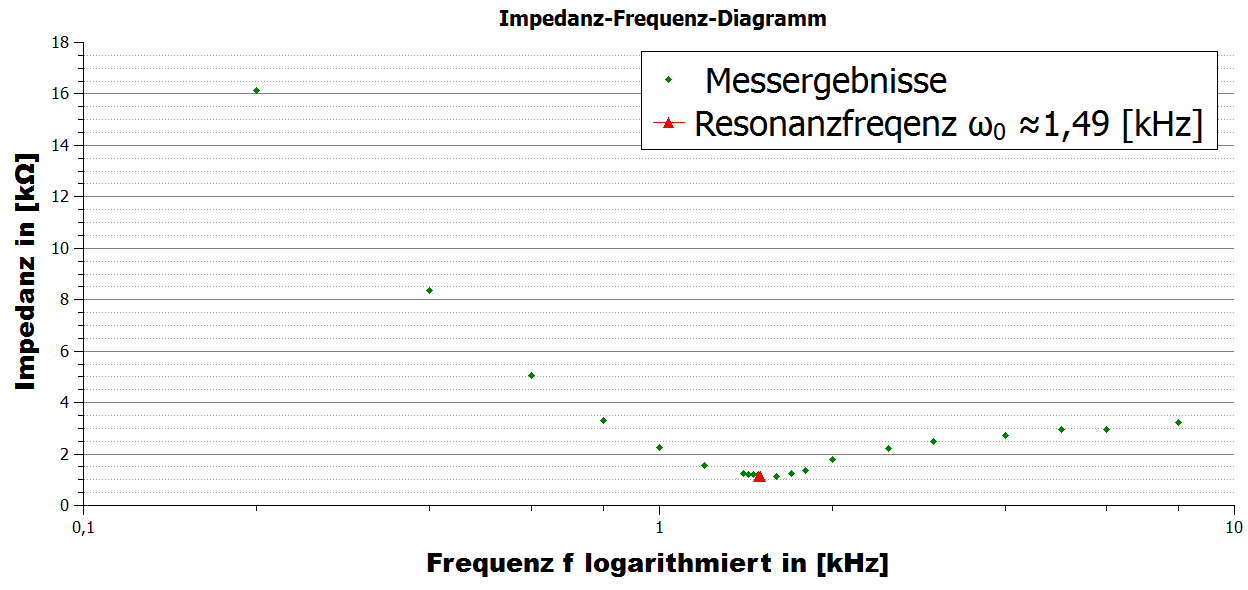
\includegraphics[scale=0.5]{Graphik/Impedanz}
\caption{Impedanz-Frequenz-Diagramm}
\end{figure}
\noindent
Mit Hilfe eine Impedanz-Frequenz-Diagramm wird nun graphisch ersichtlich, dass unsere Resonanzfrequenz etwa bei $1,49\,$kHz liegt das Minimum unserer 
Kurve ist.
Man sieht ebenfalls den Abfall der Impedanz bis zu dem Zeitpunkt der Resonanzfrequenz. Ab da steigt die Impedanz bei uns wieder leicht. Der Theorie nach 
sollte hier die Kurve parabelförmig verlaufen. Im Abschnitt Fehlerquellen erklären wir, wieso es bei uns nicht so ist.
\newpage
\subsection{Berechnung der Phasenverschiebung}
Zu guter Letzt wird noch die Phasenverschiebung die Formel (8) verwendet.
Eine Beispielrechnung wird hier wieder für $2\,$kHz ausgeführt.  
\begin{align*}
\Phi = \arctan(\frac{\Im(Z_{x})}{\Re(Z_{x})}) = \arctan(\frac{1387,26}{1093,56}) =0,9\,{\text{rad}}=51,78^{\circ}
\end{align*}
\noindent
In der folgenden Tabellen befinden sich all unsere Messwerte und berechneten Werte.
\begin{figure}[h]
\vspace{-10pt}
\centering
\caption{Messwerte}
\begin{tabular}{|c|c|c|c|c|c|c|c|} \hline
Frequenz [kHz]	&$C_n$ in [nF]& $R_n$ in $[k\Omega]$ & $\Im(Z_x) [\Omega]$ & $
\Re(Z_x) [\Omega]$ & $\mid Z_x\mid$ $[\Omega]$& Phase [$^{\circ}$]  \\ 
\hline	
0,20&	50,00		&2,50		&-15923,57		&2500,00	&16118,62 	&-81,12\\ \hline	
0,40&	50,00		&2,50		&-7961,78		&2500,00	&8345,06	&-72,60\\ \hline	
0,60&	54,00		&1,20		&-4914,68		&1200,00	&5059,06	&-76,32\\ \hline	
0,80&	64,00		&1,10		&-3110,07		&1100,00		&3298,87	&-70,56\\ \hline	
1,00&	84,00		&1,20		&-1895,66		&1200,00	&2243,55	&-57,69\\ \hline	
1,20&	133,00		&1,20		&-997,72			&1200,00	&1560,59	&-39,76\\ \hline	
1,40&	423,00		&1,20		&-268,89			&1200,00	&1229,76	&-12,64\\ \hline	
1,43&	710,00		&1,20		&-156,84			&1200,00	&1210,21	&-7,45\\ \hline	
1,46&	1100,00	&1,20		&-99,15			&1200,00	&1204,09	&-4,73\\ \hline	
1,49&	1100,00	&1,20		&-97,15			&1200,00	&1203,93	&-4,63\\ \hline	
\multicolumn{1}{c}{Resonanzfrequenz} \\ \hline
1,60&	1,00		&20,20	&277,45			&1093,56	&1128,21	&14,24\\ \hline	
1,70&	2,00		&20,20	&554,90			&1093,56	&1226,29	&26,92\\ \hline	
1,80&	3,00		&20,20	&832,35			&1093,56	&1374,30	&37,29\\ \hline	
2,00&	5,00		&20,20	&1387,25		&1093,56	&1766,45	&51,78\\ \hline	
2,50&	7,00		&20,20	&1942,15		&1093,56	&2228,87	&60,65\\ \hline	
3,00&	8,00		&20,20	&2219,60		&1093,56	&2474,37	&63,80\\ \hline	
4,00&	9,00		&20,20	&2497,05		&1093,56	&2726,02	&66,38\\ \hline	
5,00&	10,00		&22,00	&2774,50		&1004,09	&2950,61	&70,14\\ \hline	
6,00&	10,00		&22,00	&2774,50		&1004,09	&2950,61	&70,14\\ \hline	
8,00&	11,00		&22,00	&3051,95		&1004,09	&3212,88	&71,83\\ \hline	
\end{tabular} 
\end{figure}
~\\
Des weiteren ist noch ein Phasen-Frequenz-Diagramm erstellt worden. Durch fitten unserer Messwerte mit der Fitkurve $\varphi = a+ b\cdot\arctan(c[\frac{x\cdot 360}{2\pi} + d])$ in Qtiplot, die mit Hilfe von Formel (9) angesetzt wird, erkennt man, dass sich unsere Resonanzfrequenz im Nulldurchgang der gefitteten Kurve befindet. \\
\newpage
\begin{figure}[h!]
\centering
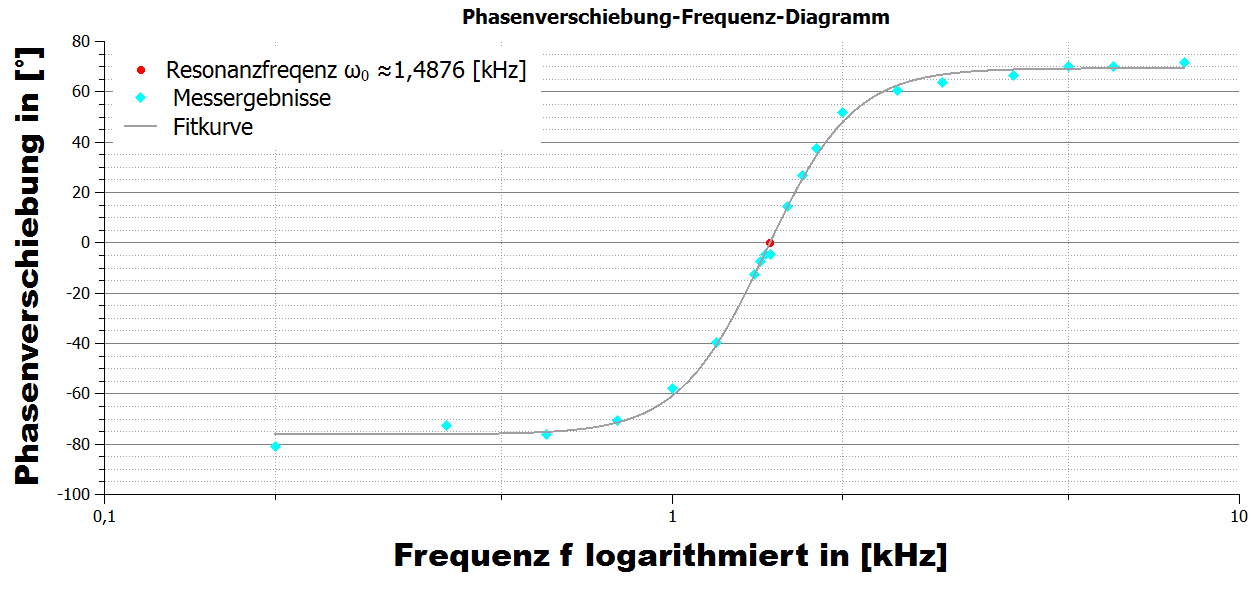
\includegraphics[scale=0.5]{Graphik/Phase}
\vspace{-10pt}
\caption{Phasen-Frequenz-Diagramm}
\end{figure}
\noindent
Werten wir die Fitkurve am Punkt $\varphi=0^{\circ}=0$\,Rad aus, so erhalten wir eine Resonanzfrequenz von $\omega_0=1,4876$\,kHz liegt. 


\section{Fehlerquellen}

Die Fehlerquellen bei der Messung lassen sich an verschieden Stellen finden. Bei höheren Frequenzen ist die Empfindlichkeit gegenüber äußeren Einflüssen 
größer. Um die äußeren Einflüsse gering zu halten, misst man optimaler Weise mit kurzen Kabeln. Die Messung unseres Versuches wurde zum Teil mit langen 
Kabeln durchgeführt, wodurch vermutlich ein nicht feststellbarer Fehler entstanden ist. \\
~\\
Die verwendeten Geräte können auch systematische Fehler in der Anzeige und der Messung haben, was zu einem Fehler beitragen kann.
Das Feststellen des Minimums ist zudem auch fehlerbehaftet, da man bei einer Frequenz zwischen 1,4 kHz und 1,6 kHz durch variieren des 
Stufenkondensators und der Widerstandsdekaden keine Veränderung des Minimums mehr erzeugen konnte. \\
~\\
Eine weitere Fehlerquelle bei uns war, dass wir selbst mit dem Stufenkondensator relativ schnell an den maximalen Einstellungen waren und variieren des ohmschen Widerstandes bei uns kaum Auswirkungen hatten, deswegen ist bei uns im Impedanz-Frequenz-Diagramm keine richtige Parabel zu erkennen.
\newpage

\section{Zusammenfassung}

Unser Ziel in dem Versuch war es zuerst, die Resonanzfrequenz zu bestimmen, welche bei uns bei $1,5\,$kHz lag. Das Impedanz-Frequenz-Diagramm stimmt 
mit der Theorie überein, dass die Resonanzfrequenz die Impedanz minimal wird. Bei der Phasenverschiebung ist erst nicht viel zu erkennen. Erst durch fitten 
der Messwerte ergab sich nicht nur deutliche ein Arkustangens, sondern es wird auch erkennbar, dass die Resonanzfrequenz ein Wendepunkt des 
Arkustangens wird. Unsere Resonanzfrequenz liegt damit bei etwa $\omega_0=1,4876$\,kHz.

\section{Literaturverzeichnis}

\begin{thebibliography}{xxxxxxxx}
	\bibitem[1]{1}		\textit{\glqq E10 Wechselstromwiderstände: Serienschwingkreis\grqq , in 
								http:www3.physik.uni-stuttgart.de/studium/praktika/ap/},\textit{ unter 
								http://www3.physik.uni-stuttgart.de/studium/praktika/ap/pdf\_dateien/E10.pdf abgerufen am 1.05.2015}
   \bibitem[A]{A}  	Graphik aus \textit{\glqq E10 Wechselstromwiderstände: Serienschwingkreis\grqq , in 	http://www3.physik.uni-stuttgart.de/studium/
   								praktika/ap/}, \textit{ unter 	http://www3.physik.uni-stuttgart.de/studium/praktika/ap/pdf\_dateienE10.pdf  Seite 7; abgerufen am 1.05.2015} 
	\bibitem[B]{B}  	Graphik aus \textit{\glqq E10 Wechselstromwiderstände: Serienschwingkreis\grqq , in 	http://www3.physik.uni-stuttgart.de/studium/
   								praktika/ap/}, \textit{ unter 	http://www3.physik.uni-stuttgart.de/studium/praktika/ap/pdf\_dateienE10.pdf Seite 8; abgerufen am 1.05.2015}

\end{thebibliography}

\section{Anhang}

\begin{figure}[h]
\vspace{-20pt}
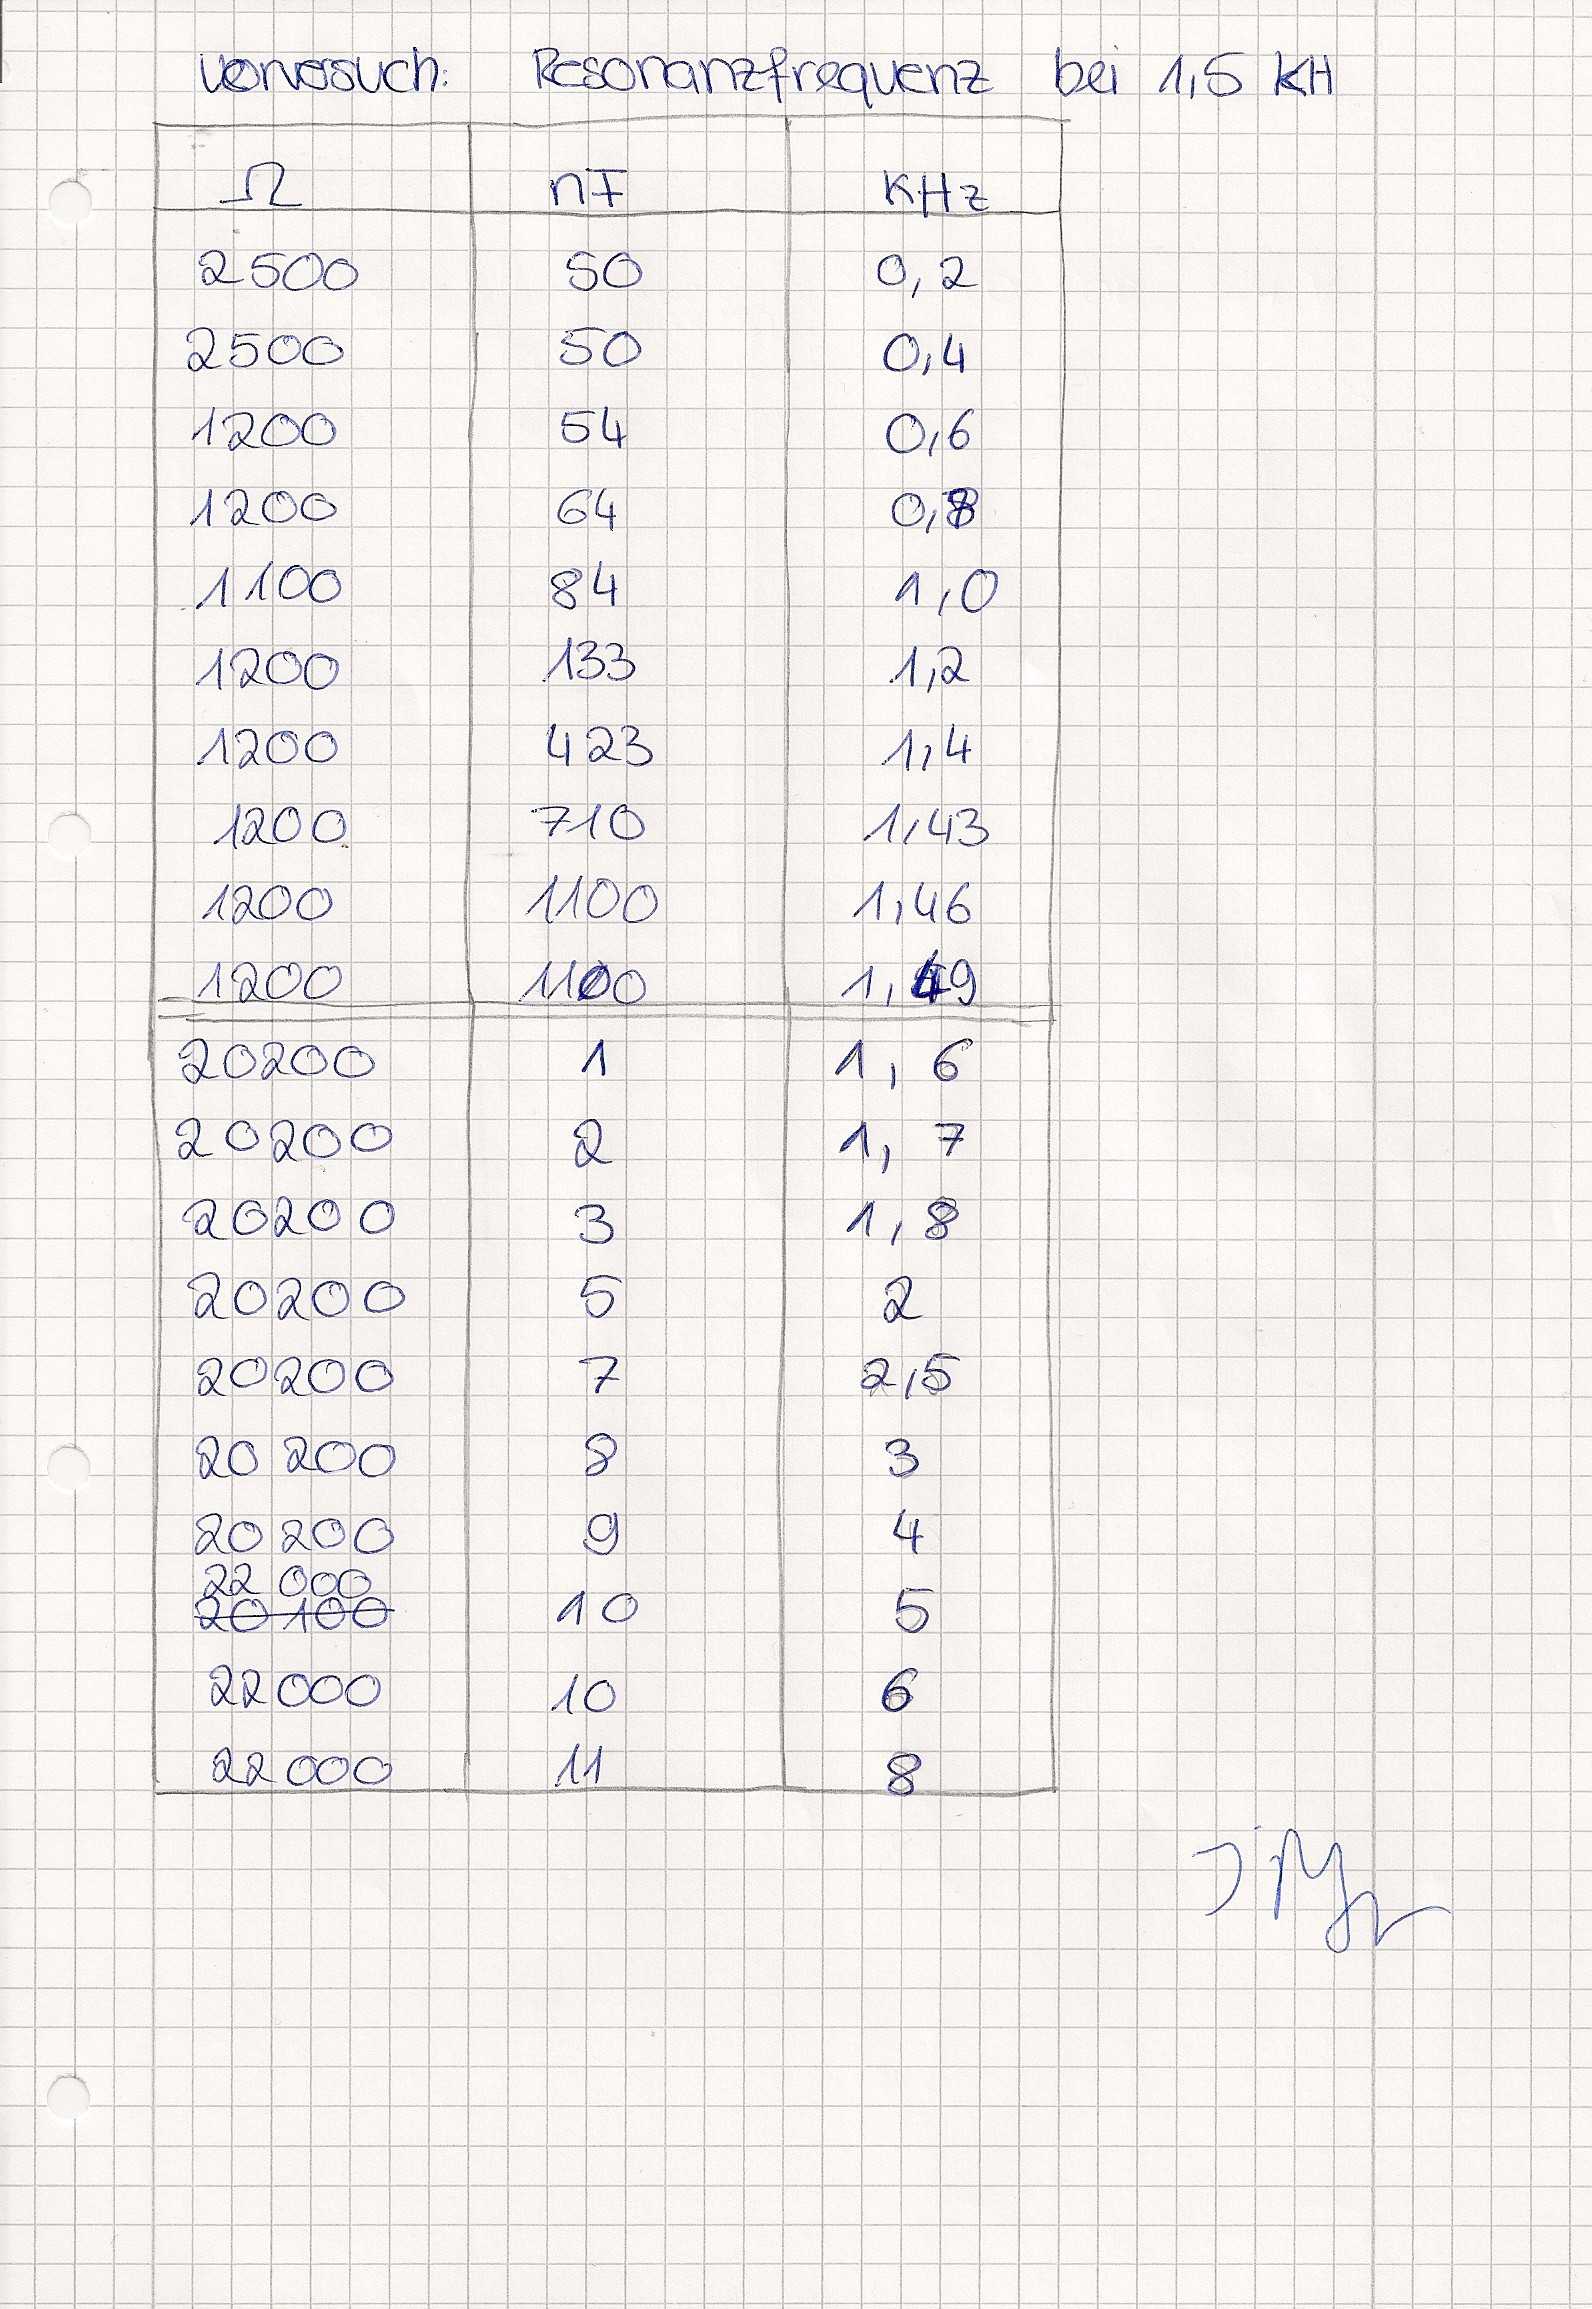
\includegraphics[scale=0.3]{Graphik/Linda}
\end{figure}

\end{document}